\documentclass[10pt,a4paper]{article}
\usepackage[utf8]{inputenc}
\usepackage{amsmath}
\usepackage{graphicx}
\usepackage{amsfonts}
\usepackage{hyperref}
\usepackage{amssymb}
\author{Cosimo Damiano Persia\\cpersia@unibz.it}
\title{KRO - PROJECT\\Pizza class recognizer}
\begin{document}
\maketitle

\section{Domain of choice}
The domain of choice of this project is a pizza shop 2.0 . The software is aimed to a new kind of pizza shop completely automated by machines. The users creates its own pizza by selecting the ingredients from an user interface.  The software, using the information of the ingredients inserted by the user, simulates the pizza, recognizes the class which the pizza belongs to and it outputs the result. In this way, customers have a direct feedback and maybe a suggestion of the food they will be eating. If the users do not like the classification of the pizza they have chosen, they can modify the ingredients. 
The owner of the restaurant can ask additional queries. The software supports the query that asks what pizzas a specific class of user bought. In this way the owner (or the machine) can understand what are the best pizzas to propose in a specific period of the year and buy the correct ingredient in order to make the expected pizzas. 


\section{Database}
The database contains the information of users who have bought a pizza.
The software uses information from a database with the schema shown in figure \ref{DBSCHEMA}.

\begin{figure}
  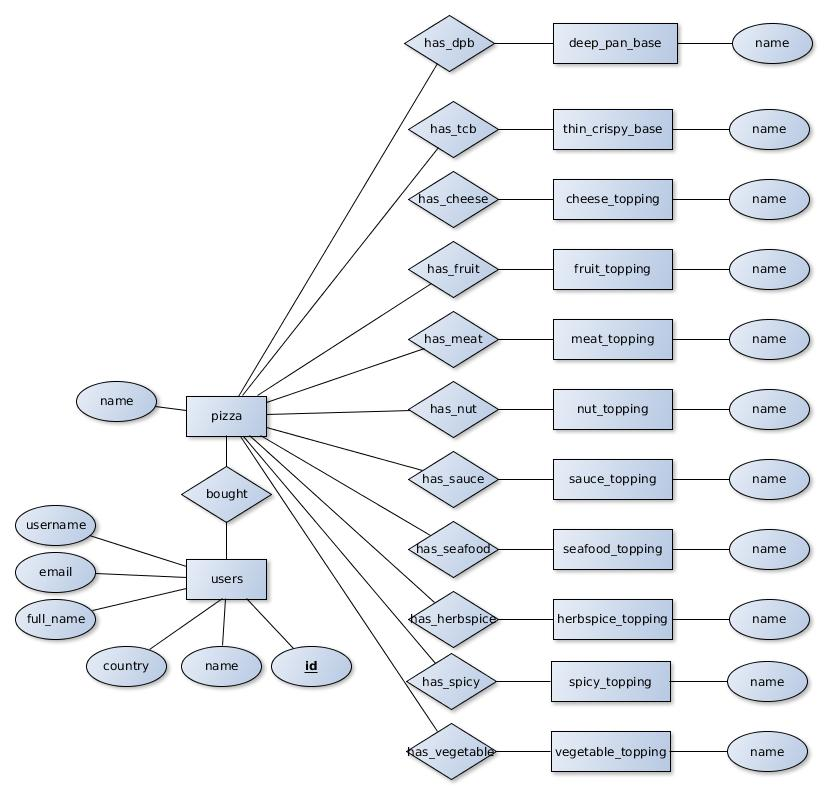
\includegraphics[width=\linewidth]{database_schema.jpg}
  \caption{Database ER diagram}
  \label{DBSCHEMA}
\end{figure}

For each user the username, email, full name, country, name, and id are stored and for the pizza only its name is stored. 
Each pizza has a type of dough that can be "deep pan"  or "thin and crispy". Moreover each pizza can have unrestricted numbers of vegetable, spicy, herb, seafood, sauce, nut, meat, fruit or cheese toppings.

The database contains a wide variety of ingredients of every kind; on average the size of each table representing the type of an ingredient is 1 MB. The size of the database on the whole is 29 MB. The data of the ingredients has been downloaded from multiple websites which had food and health as their primary domain. 

\section{Ontology}
The ontology was deisgned using Protege \footnote{\url{https://protege.stanford.edu/}}, and it represents the hierarchy of classes of pizza and topping. Starting from the basic pizzas distinguished by the raw ingredients in bottom, new classes of pizza are stated. 
The ontology contains more or less 50 concepts and 12 roles. The mapping between the ontology and the database are 23. One for each type of ingredient and one for the corresponding pizza with that ingredient. For example a pizza for carnivores (CarnivorePizza in the ontology) is a pizza that contains meat (MeatyPizza) or Fish (SeaFood).  The database does not know anything about the hierarchy of pizza and the database stores only the raw information.

A graphical representation of the ontology is shown in figure \ref{ONTO} .
\begin{figure}
  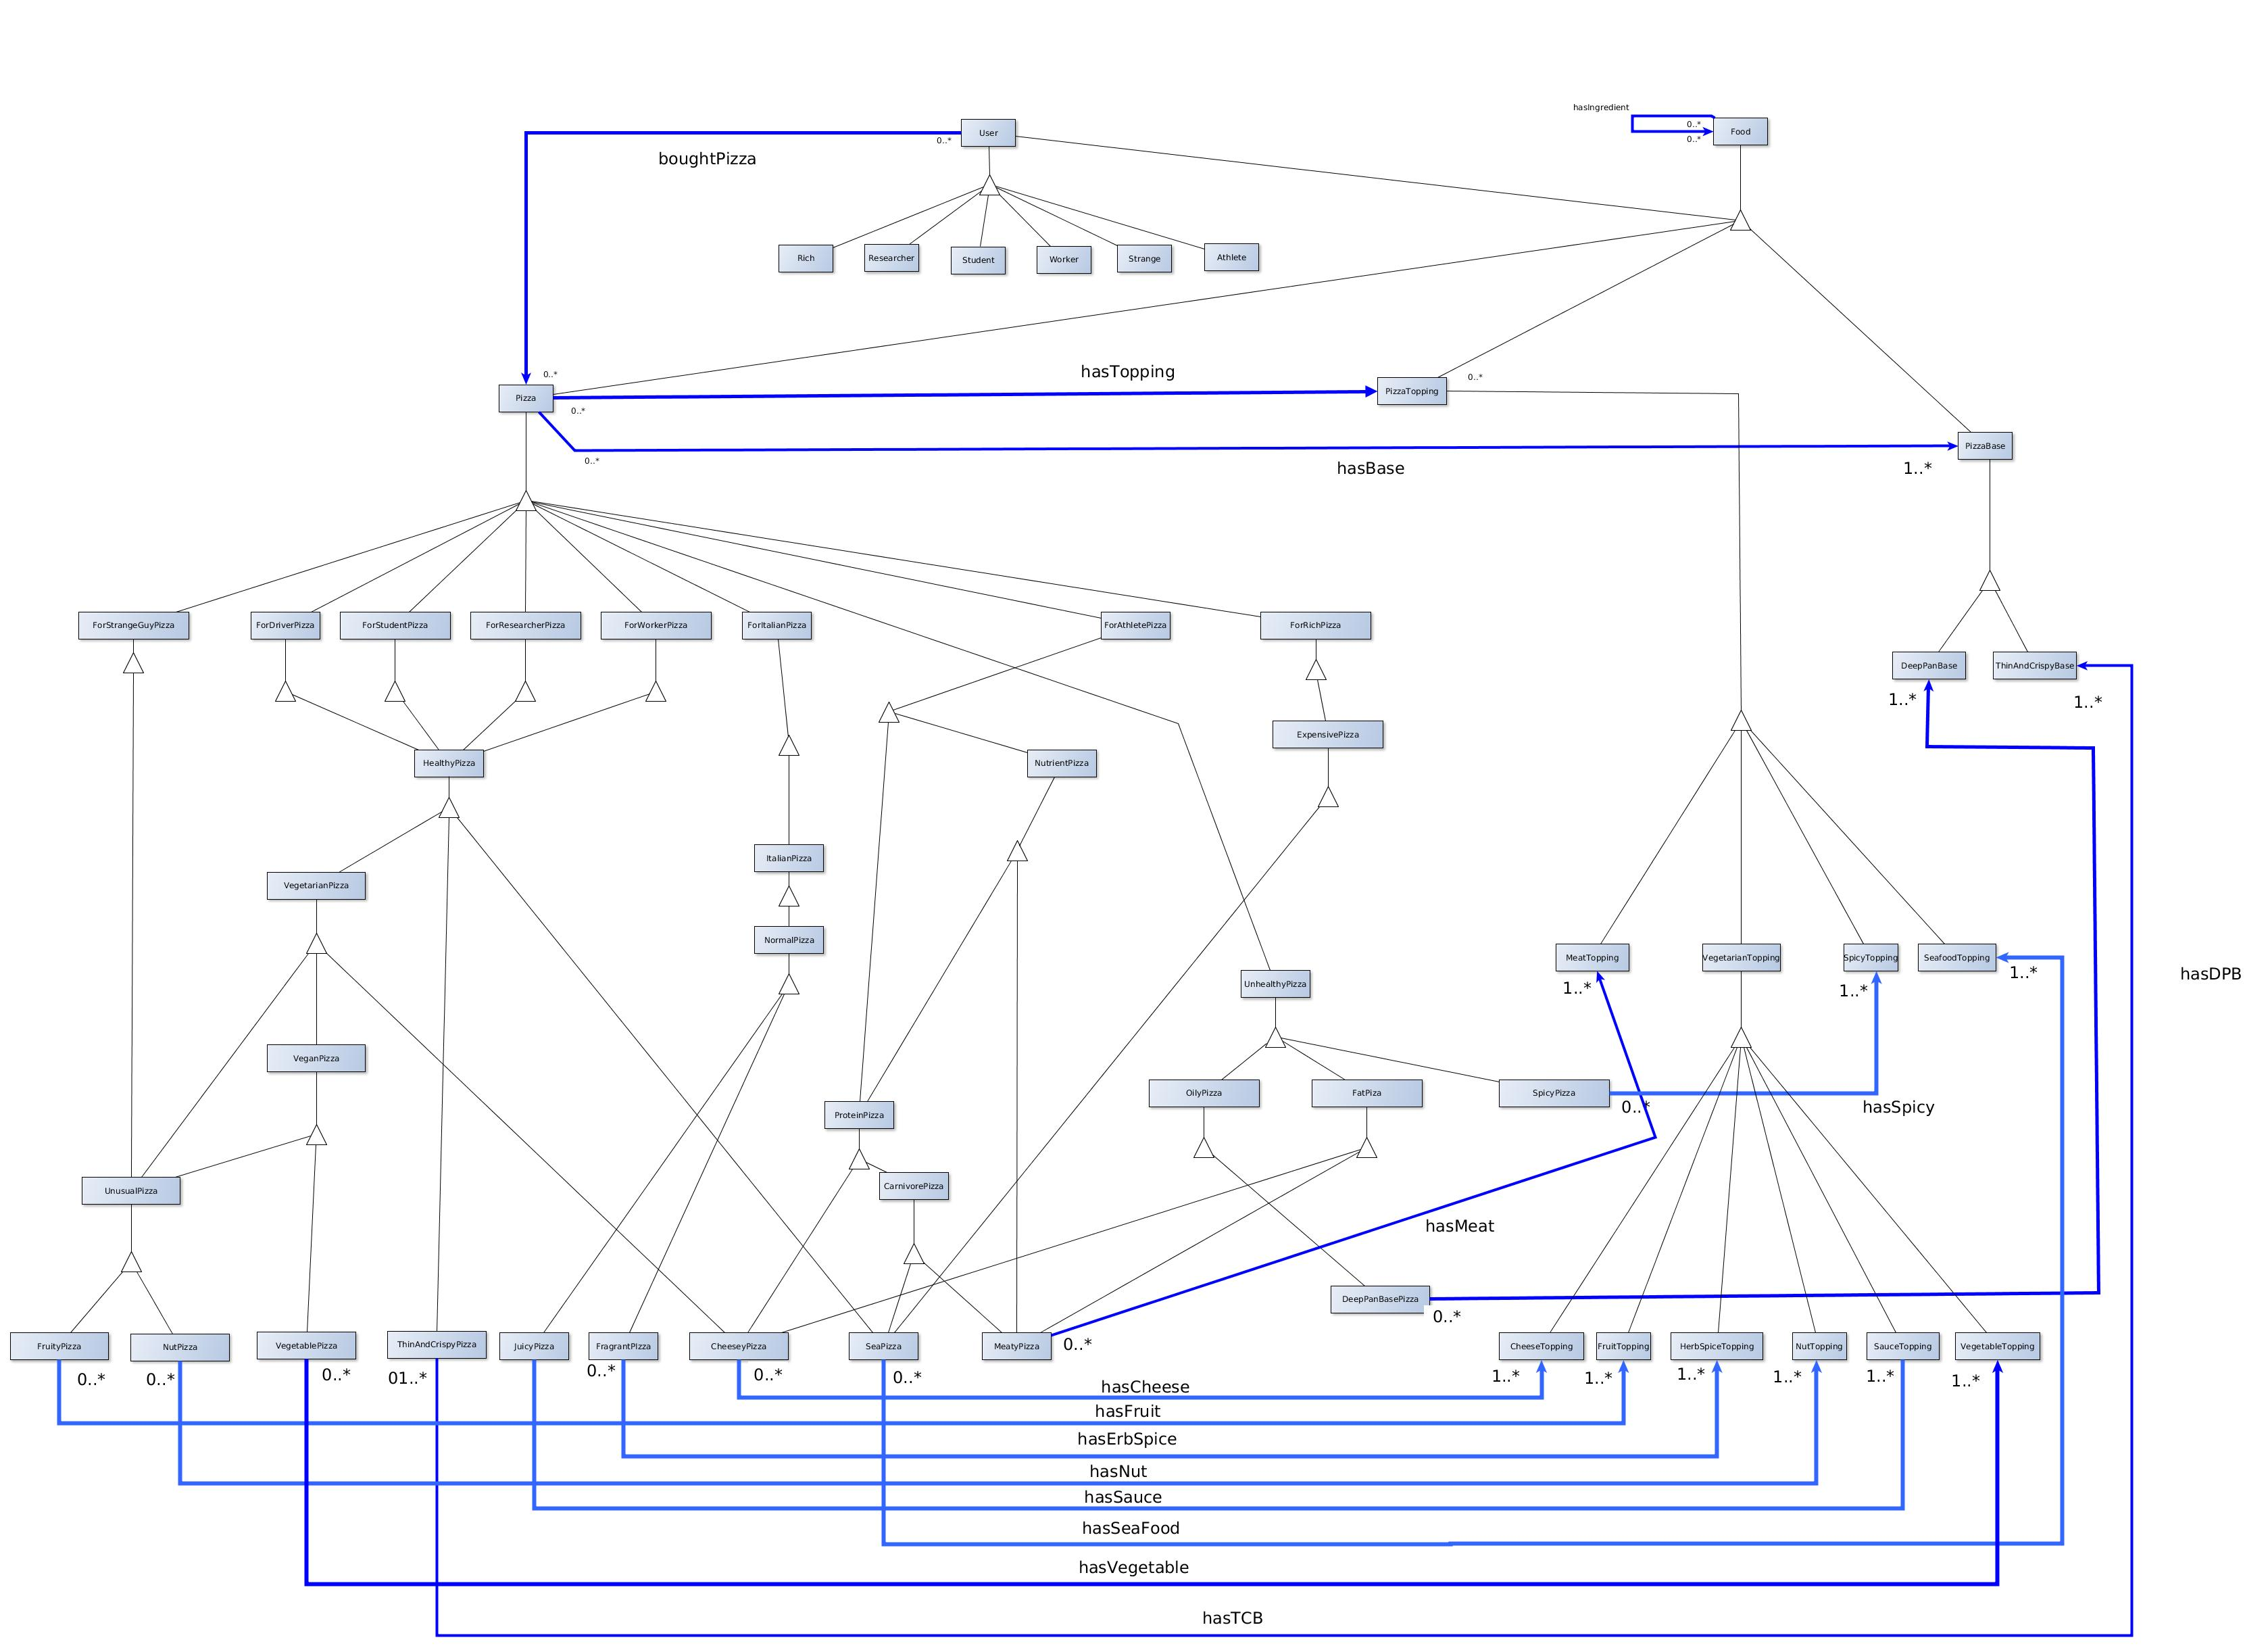
\includegraphics[width=\linewidth]{ontologygraph.jpg}
  \caption{Ontology graphical representation}
  \label{ONTO}
\end{figure}

\section{SOFTWARE}
The software uses the framework ONTOP \footnote{\url{https://github.com/ontop/ontop}} to link the information of the database and the ontology. The connection is made by writing mappings. As an example the following mapping links the concept CheeseTopping with the information stored in the database in the table "cheese\_topping".
\begin{center}
target		:\{name\} a :pizza\#{CheeseTopping} .  \\
source		select name from cheese\_topping
\end{center}

The following mapping links the relation in the database has\_cheese with the relation in the ontology "hasCheese".
\begin{center}
target		:\{name\_pizza\} :pizza\#{hasCheese} :\{name\} .  \\
source		select name\_pizza, name from has\_cheese
\end{center}

The software needs to connect to a Postgresql database \footnote{\url{https://www.postgresql.org/}} and in order to do so it needs the corresponding driver \footnote{\url{https://jdbc.postgresql.org/}} to establish a connection. As mentioned before, the software uses the ONTOP framework to query the database and to use the ontology. In order to provide a graphical user interface, the javafx library has been chosen \footnote{\url{http://www.oracle.com/technetwork/java/javase/overview/javafx-overview-2158620.html}} and in order to supply autocompletion, during the insertion of ingredients, the controlfx library has been used.

\end{document}